\section*{Introduction}
The prefrontal cortex (PFC) has been implicated in executive functions, such as planning, decision making, working memory, emotional modulation and control of social behavior. Damages to the PFC are associated to impairment of these functions in psychiatric disorders, including schizophrenia and attention-deficit/hyperactivity disorder (\cite{wise08for,kandel13pri,bang18dis}). \\

Our comprehension in different fields of neuroscience has been continuously increasing through numerous areas of research. Nevertheless, our understanding of the computational and dynamic properties of the brain, and the PFC in particular, is still limited. In this regard, computational network models are invaluable tools for probing such properties as they enable us to meaningfully integrate data from different fields.\\

Based on experimental data, Hass et al. \cite{Hass2016} developed a computational network model of the PFC with physiological validity and predictive capability at both the single-neuron and the network levels. The original implementation, available on ModelDB (\cite{ModelDB}), used MATLAB for the network setup and C for the actual simulation. In this work, we reimplemented the model using Python and the Brian 2 simulator (\cite{stimberg19bri}). We also performed tests and analyzed the results similarly to the the original work, besides identifying and discussing aspects that were not explicitly specified there.\\

\section*{Methods}
In this section, we detail the network model, the reimplementation and the tests and analyses we performed. Henceforth we will refer to simulations without any applied stimuli as baseline simulation, and to simulations with stimulation protocols as test simulation. In order to exclude transient dynamics, we applied stimuli and performed analyses always after 1 second of simulation.\\

As in the original work, we call neurons with more than 10 spikes in 30 s of baseline simulation `spiking neurons'. \\

\subsection*{Network structure}

The model was built mainly upon data from experiments with rodents, with the addition, when rodent data were scarce, of results obtained from cats, monkeys and ferrets. It consists of a column with 1000 neurons organized into a bilaminar structure made of layer 2/3 (L2/3) and layer 5 (L5). Layer 4 is absent in the rodent PFC; layer 1 is mostly composed by long-range fiber bundles; and layer 6 is weakly connected to the other layers; therefore they were omitted.\\

The neurons are of two types: excitatory pyramidal cells (PC) and inhibitory interneurons (IN). In each layer, the interneurons are subdivided into local interneurons (IN-L0), which are fast-spiking cells; cross-layer interneurons (IN-CL0), which are bitufted cells; cross-column interneurons (IN-CC), which are large basket cells; and far-reaching interneurons (IN-F), which are Martinotti cells. As defined in the original code, each one of the first two groups was further subdivided into two subgroups (IN-L0 into IN-L/IN-L-d and IN-CL0 into IN-CL/IN-CL-AC) according to the latency time and the spike rate, respectively. The proportion of cells in each group is specified in Table \ref{tab:tab1}. \\

\begin{table}
    \centering
    \begin{tabular}{|c|c|c|c|c|c|c|c|} 
     \hline
     \diagbox{Layer}{Group} & PC & IN-L & IN-L-d & IN-CL & IN-CL-AC & IN-CC & IN-F \\[2pt]
    \hline\hline
   L2/3  & 47\% & 1.55\% & 1.55\% & 1.3\% & 1.5\% & 2.6\% & 2.1\% \\[1pt]
    \hline
    L5 & 38\% & 0.25\% & 0.25\% & 0.25\% & 0.25\% & 1.8\% & 1.8\%\\[1pt]
    \hline
    
    \end{tabular}
    \caption{Proportion of cells in each neuron group.}
    \label{tab:tab1}
\end{table}

The probability of connection between each pair of neurons is set according to the pre- and post-synaptic groups they pertain to (Tables \ref{tab:tab2} and \ref{tab:tab3}). The intrinsic connections among L2/3 and L5 PC neurons follow a rule so that the probability of connection increases linearly with the number of neighbors that both cells share. The proportion of reciprocity among these connections is set to 47\%. Although discussed in the article and built on the original code, this neighborhood rule is not functional in the original model due to matrices mismatches.\\

The original model as well as our reimplementation enables simulations with more columns, although the main analyses that were performed used only one. Except for intercolumn connections, distance between pairs of neurons is not defined, and the distribution of synaptic parameters and probabilities depend solely on the pre- and post-synaptic groups.\\
\begin{table}
    \centering
    \resizebox{\columnwidth}{!}{%
    \begin{tabular}{|c|c|c|c|c|c|c|c|c|} \hline
     \multicolumn{2}{|c|}{\multirow{2}{*}{\diagbox{Post-}{Pre-}}}& \multicolumn{7}{|c|}{L2/3} \\[1pt]    \cline{3-9}
     \multicolumn{2}{|c|}{} & PC & IN-L & IN-L-d & IN-CL & IN-CL-AC & IN-CC & IN-F\\    \hline\hline
     \multirow{7}{*}{L2/3}& PC & 13.93\% & 45.86\% & 45.86\% & 41.64\% & 41.64\% & 45.86\% & 67.65\% \\[1pt]     \cline{2-9}
     &IN-L & 32.47\% & 25.00\% & 25.00\% & 25.00\% & 25.00\% & 25.00\% & 25.00\%  \\[1pt]     \cline{2-9}
      &IN-L-d & 32.47\% & 25.00\% & 25.00\% & 25.00\% & 25.00\% & 25.00\% & 25.00\% \\[1pt]     \cline{2-9}
     &IN-CL & 15.94\% & 25.00\% & 25.00\% & 25.00\% & 25.00\% & 25.00\% & 25.00\%  \\[1pt]     \cline{2-9}
      &IN-CL-AC & 15.94\% & 25.00\% & 25.00\% & 25.00\% & 25.00\% & 25.00\% & 25.00\% \\[1pt]     \cline{2-9}
     &IN-CC & 32.47\% & 25.00\% & 25.00\% & 25.00\% & 25.00\% & 25.00\% & 25.00\%  \\[1pt]     \cline{2-9}
      &IN-F & 29.00\% & 25.00\% & 25.00\% & 25.00\% & 25.00\% & 25.00\% & 25.00\% \\
      \hline\hline
     \multirow{7}{*}{L5}& PC & 23.33\% & 21.30\% & 21.30\% & 19.34\% & 19.34\% & 21.30\% & 31.42\% \\[1pt]     \cline{2-9}
     &IN-L & 32.47\% & 0 & 0 & 0 & 0 & 0 & 0 \\[1pt]     \cline{2-9}
      &IN-L-d & 32.47\% & 0 & 0 & 0 & 0 & 0 & 0 \\[1pt]     \cline{2-9}
     &IN-CL & 15.94\% & 0 & 0 & 0 & 0 & 0 & 0 \\[1pt]     \cline{2-9}
      &IN-CL-AC & 15.94\% & 0 & 0 & 0 & 0 & 0 & 0 \\[1pt]     \cline{2-9}
     &IN-CC & 32.47\% & 0 & 0 & 0 & 0 & 0 & 0 \\[1pt]     \cline{2-9}
      &IN-F & 29.00\% & 0 & 0 & 0 & 0 & 0 & 0 \\
      \hline
     \end{tabular}%
     }
    \caption{Connection probabilities from pre-synaptic L2/3 groups to all post- synaptic groups.}
    \label{tab:tab2}
\end{table}


\begin{table}
    \centering
    \resizebox{\columnwidth}{!}{%
    \begin{tabular}{|c|c|c|c|c|c|c|c|c|} \hline
     \multicolumn{2}{|c|}{\multirow{2}{*}{\diagbox{Post-}{Pre-}}}& \multicolumn{7}{|c|}{L5} \\[1pt]    \cline{3-9}
     \multicolumn{2}{|c|}{} & PC & IN-L & IN-L-d & IN-CL & IN-CL-AC & IN-CC & IN-F\\    \hline\hline
     \multirow{7}{*}{L2/3}& PC & 4.49\% & 9.91\% & 9.91\% & 3.21\% & 3.21\% & 9.91\% & 12.87\% \\[1pt]     \cline{2-9}
     &IN-L & 18.75\% & 0 & 0 & 0 & 0 & 0 & 0 \\[1pt]     \cline{2-9}
      &IN-L-d  & 18.75\% & 0 & 0 & 0 & 0 & 0 & 0\\[1pt]     \cline{2-9}
     &IN-CL  & 9.20\% & 0 & 0 & 0 & 0 & 0 & 0 \\[1pt]     \cline{2-9}
      &IN-CL-AC & 9.20\% & 0 & 0 & 0 & 0 & 0 & 0\\[1pt]     \cline{2-9}
     &IN-CC  & 18.75\% & 0 & 0 & 0 & 0 & 0 & 0 \\[1pt]     \cline{2-9}
      &IN-F  & 16.74\% & 0 & 0 & 0 & 0 & 0 & 0\\
      \hline\hline
     \multirow{7}{*}{L5}& PC & 8.06\% & 70.06\% & 70.06\% & 22.71\% & 22.71\% & 70.06\% & 90.96\% \\[1pt]     \cline{2-9}
     &IN-L & 18.75\% & 60.00\% & 60.00\% & 60.00\% & 60.00\% & 60.00\% & 60.00\% \\[1pt]     \cline{2-9}
      &IN-L-d & 18.75\% & 60.00\% & 60.00\% & 60.00\% & 60.00\% & 60.00\% & 60.00\%\\[1pt]     \cline{2-9}
     &IN-CL & 9.20\% & 60.00\% & 60.00\% & 60.00\% & 60.00\% & 60.00\% & 60.00\%\\[1pt]     \cline{2-9}
      &IN-CL-AC  & 9.20\% &60.00\% & 60.00\% & 60.00\% & 60.00\% & 60.00\% & 60.00\%\\[1pt]     \cline{2-9}
     &IN-CC  & 18.75\% & 60.00\% & 60.00\% & 60.00\% & 60.00\% & 60.00\% & 60.00\% \\[1pt]     \cline{2-9}
      &IN-F  & 16.74\% & 60.00\% & 60.00\% & 60.00\% & 60.00\% & 60.00\% & 60.00\%\\
      \hline
     \end{tabular}%
     }
    \caption{Connection probabilities from pre-synaptic L5 groups to all post- synaptic groups.}
    \label{tab:tab3}
\end{table}

\subsection*{Neurons}

The network neurons follow the simplified adaptive exponential intergrate-and-fire (simpAdEx) model (\cite{hertag12ana}). The simpAdEx model derives from the adaptive exponential integrate-and-fire (AdEx) (\cite{brette05ada}) model through a time-scale separation that enables closed-form expressions for transient and stationary firing rates. \\

The two-dimensional internal state of the neuron is described by the membrane voltage \textit{V} and the adaption current \textit{w} and evolves according to

\begin{subequations}
\label{eq:Membrane}
\begin{align}
    C \frac{dV}{dt} &= - g_{L} \cdot (V - E_{L}) + g_{L} \cdot \Delta_{T} \cdot e^{\frac{V - V_{T}}{\Delta_{T}}} + I - w := w_V - w,\label{eqn:dvdt}\\
    \tau_w \frac{dw}{dt}  &=
\begin{cases}
    0, & \text{if } \tau_m \cdot w_V < \tau_w \cdot |w - w_V |\\
    \Theta (V_T - V) \cdot \left[ 1 - \frac{\tau_m}{\tau_w}\right] \frac{dw_V}{dV}\frac{dV}{dt},              & \text{otherwise},
    \end{cases} \label{eqn:dwdt}
\end{align}
\begin{align}
&\text{If } V = V_{\text{up}} \Rightarrow V \rightarrow V_{r} \text{ and } w \rightarrow w + b \text{,}\\ 
&\text{If} \left( 1 - \frac{\tau_m}{\tau_w} \right) w_V < w <  \left( 1 + \frac{\tau_m}{\tau_w} \right)w_V \Rightarrow w = \left( 1 - \frac{\tau_m}{\tau_w} \right) w_V,\\
&\text{with } \tau_m = \frac{C}{g_L} \nonumber
\end{align}
\end{subequations}

where capacitance \textit{C}, conductance $g_L$, reversal potential $E_L$, voltage threshold $V_T$, threshold slope factor $\Delta_T$, adaptation membrane constant $\tau_w$, reset trigger voltage $V_{\text{up}}$, reset voltage $V_r$ and reset \textit{w}-increment \textit{b} are membrane parameters, $\tau_m = \frac{C}{g_L}$ is the membrane time constant, $w_V$ is the the \textit{w} value over the \textit{V}-nullcline, $\Theta$ is the Heaviside function and \textit{I} is the total current. \textit{I} is given by
\begin{equation}
I = I_{\text{inj}} + I_{\text{syn}} = I_{\text{inj}} + \sum_{X \in \text{Recep}} I_X, \text{ \\with } \text{Recep} = \{\text{AMPA, GABA}_A\text{, NMDA}\}
\label{eqn:currents}
\end{equation}
where the synaptic current $I_{\text{syn}}$ is the sum of currents due to AMPA, GABA$_A$ and NMDA receptors and $I_{\text{inj}}$ corresponds to further stimuli applied directly to the neuron and accounts for the background current described below. For each neuron group, the membrane parameters are drawn from multivariate Gaussian distributions through a Box-Cox transformation, since some of their individual distributions are non Gaussian. The parameters of the Gaussian distributions for each neuron type are listed in Table~\ref{tab:membparams}.\\

Whenever $V$ crosses $V_{\text{up}}$ a spike is recorded, $V$ is reset to $V_r$ and  $w$ is reset to $w + b$. As implemented in the original code itself, if $w$ gets close to $w_V$ so that $w_V - D(V) < w < w_V + D(V)$, $w$ is reset to $w_V – D(V)$. Although the original text describes the reset condition only as $w$ crossing $w_V + D(V)$, other $w$ values in the interval from $w_V – D(V)$ to $w_V + D(V)$ may come up right after the spike reset and would generate inconsistent behaviors if they got too close to $w_V$ due to the singularity of equations (\ref{eqn:dvdt}) and (\ref{eqn:dwdt}) over the $V$-nullcline.\\

From equation (\ref{eqn:dvdt}), we derive

\begin{equation}
I_{SN} = g_L \cdot (V_T - E_L - \Delta_T), 
\label{eqn:rheobase}
\end{equation}

where $I_{SN}$ is the rheobase current, which depends solely on $g_L$, $V_T$, $E_L$ and $\Delta_T$.\\

Despite not discussed in the original text, the original code and our reimplementation define the refractoriness of 5 ms after each spike. During the refractory period, the neuron is not allowed to spike. Regarding the refractory subthreshold dynamics, for each neuron a refractory current ($I_{\text{ref}}$) is defined as the total current that leads to a transient frequency of 200 Hz. In the refractory period, if $I<I_{\text{ref}}$, $V$ evolves according to equation (\ref{eqn:dvdt}). Otherwise, if $I \geq I_{\text{ref}}$, $V$ is driven exponentially back to $V_r$.\\


\subsection*{Synapses}

Neurons are connected through conductance-based inhibitory GABA$_A$ and excitatory AMPA and NMDA synapses that are additionally modulated by short-term plasticity (STP) and affected by a failure rate of 30\%. The AMPA, GABA$_A$ and NMDA conductances are given by 

\begin{align}
g_X(t) &= g_X^{\text{max}} \left( \sum\limits_{t_{\text{sp}}} a(t_{\text{sp}}) \left( \text{exp}\left(- \frac{t - t_{\text{sp}} - \tau_D}{\tau_{\text{off}}^X}\right) - \text{exp}\left(- \frac{t - t_{\text{sp}} - \tau_D}{\tau_{\text{on}}^X}\right) \right) \right), \label{eqn:conductance}\\
\text{with }& X\in \text{\{AMPA, GABA$_A$, NMDA\}}, \nonumber
\end{align}

where maximum conductance $g_X$ and synaptic delay $\tau_D$ are parameters drawn from normal distributions specific for each pre- and postsynaptic group pair and each synaptic type, onset $\tau_{\text{on}}$ and offset $\tau_{\text{off}}$ time constants have fixed values for each synaptic type; $\{t_{\text{sp}}\}$ comprises the set of pre-synaptic spike times and $a$ is the STP parameter described below. The AMPA, GABA$_A$ and NMDA conductances of each neuron evolve according to the sum of the perturbations caused by all presynaptic spikes, excluding the failed ones.\\

The synaptic current $I_{\text{syn}}$ of each neuron is given by the sum of AMPA, GABA$_A$ and NMDA currents, which follow

\begin{subequations}
\begin{align}
I_X &= g_X(t) \cdot S(V) \cdot  (V - E_X), \label{eqn:current} \\
S(V)  &=
\begin{cases}
    \text{1.08}(1 + \text{0.19}  \exp{(-\text{0.064} V))}^{-1}, & \text{if } X = \text{NMDA}\\
    1,              & \text{otherwise,}
\end{cases}\\
X &\in \text{\{AMPA, GABA$_A$, NMDA\}}, \nonumber
\end{align} 
\end{subequations}

where $E_X$ is the reversal potential characteristic of each synaptic type  (0 mV for AMPA and NMDA and $-70$ mV for GABA$_A$) and S is a function that accounts for the effect of the magnesium ion over NMDA synapses (\cite{jahr90vol}).\\

STP models the variation in availability and efficiency of resources in each synapse after consecutive presynaptic spikes according to (\cite{maas02syn})

\begin{subequations}
\begin{align}
R_{k+1} &= 1 - (1 - (R_{k} - u_{k}  R_{k})) \cdot \text{exp}\left(-\frac{\Delta t_{k}}{\tau_{\text{rec}}}\right),\\
u_{k+1} &= U + u_{k}(1 - U) \cdot \text{exp}\left(-\frac{\Delta t_{k}}{\tau_{\text{fac}}}\right),\\
a_{k+1} &= u_{k+1} R_{k+1} ,
\end{align}
\end{subequations}

where the initial synaptic efficiency $U$ and the facilitatory $\tau_{\text{fac}}^{\scaleto{X}{3pt}}$ and recovery $\tau_{\text{rec}}^{\scaleto{X}{3pt}}$ time constants are parameters drawn from normal distributions for each pre- and postsynaptic group and specific for each synapse type (X $\in$ \{AMPA, GABA$_A$, NMDA\} ) (see Table 4 of the original article), and the synaptic efficiency $u$ and the resource availability $R$ evolve iteratively after each spike, including the failed ones.

\subsection*{Background current}

The model assumes that the cortical column is located in and receives stimuli from a larger network that is not explicitly included in the model. As a substitute to the stimuli that would come from this surrounding structure, each neuron receives a constant background current. Indicated in equation (\ref{eqn:currents}) as $I_{\text{inj}}$, the background current is estimated as values that can be generated by the surrounding structure and that can drive the column to \textit{in-vivo}-like activity. Thus, $I_{\text{inj}}$ was set to 250 pA for PC and 200 pA for IN neurons in the original work as well as in ours.\\

\subsection*{Stimulation protocols}

In order to test the network response to extrinsic stimulation, we generated regular and Poisson excitatory spike trains from neurons not explicitly simulated. For the regular spike trains, all target neurons are stimulated simultaneously by the same spike train with constant spike interval and null failure rate. The regular stimulation is specified by the total number of spikes, the stimulation interval, the synaptic strength, the target group and the fraction of stimulated neurons. For the Poisson spike trains, the stimuli are specified by the mean firing rate, the duration of stimulation, the number of neurons generating spikes, the probability of connection to target cells, the target group and the synaptic strength. The failure rate was set to 30\%. In both cases, after each extrinsic spike the stimulated neuron receives an excitatory current as in (\ref{eqn:current}) with AMPA and NMDA conductances that vary as in (\ref{eqn:conductance}). Table \ref{tab:parm_stim} contains the parameters for regular and Poisson stimulations. STP parameters of stimulated neurons are equally affected by extrinsic stimulation and intrinsic connections. \\

\begin{table}
    \centering
    \begin{tabular}{|c|c|c|} 
     \hline
      & Regular & Poisson \\[2pt]
    \hline\hline
    Target  & PC L2/3 or L5 & PC L2/3 or L5 \\[1pt]
    \hline
    Firing rate & - & 30Hz \\[1pt]
    \hline
    Spike count  & 250 or 300 & - \\[1pt]
    \hline
    Duration  & 5 ms & 100 ms \\[1pt]
    \hline
    Synaptic strength  & 0.1 nS & 2 nS \\[1pt]
    \hline
    Generating neurons  & 1 & 100 \\[1pt]
    \hline
    Connection probability  & 10\% & 10\% \\[1pt]
    \hline
    Failure rate  & 0 & 30\% \\[1pt]
    \hline
    \end{tabular}
    \caption{Parameters of stimulation protocols.}
    \label{tab:parm_stim}
\end{table}

\subsection*{Simulation}

We used Python (version 3.6.8) for setting up the network parameters and connectivity, and the Brian 2 simulator (version 2.3)  for the actual simulation.  The original model used the Runge-Kutta 2nd order method with adaptive time-step for numerical integration. However, since the Brian 2 algorithm that implements this method -- gsl\_rk2 (\cite{gslrk2}) -- is still experimental, we used the Runge-Kutta 4th order method with time step of 0.05 ms for baseline simulations and 0.01 ms for test simulations, and reproduced some results with the gsl\_rk2 algorithm for comparisons. \\

\subsection*{Analyses}

We calculated the fraction of spiking and non-spiking neurons and compared their membrane and synaptic parameters. As some parameters do not follow Gaussian distributions, we used the Mann-Whitney U-test to compare spiking and non-spiking neuron parameters with significance of 0.05. We also compared probabilities of connection between spiking and non-spiking neurons with the chi-squared test with significance of 0.05. The spiking activity in all simulations was depicted via raster plots.\\

In order to analyze the subthreshold voltage behavior of a single neuron, we extracted the spike events from voltage traces. To do so, we first estimated the subthreshold voltage fluctuation range and then removed the voltage values between the moments when $V$ crossed $V_T$ from below and voltage reset.\\

For each simulated neuron, we recorded the spike times $t_k$, $k = 1, \ldots$, and defined the interspike intervals (ISIs) as $T_k = t_{k+1} - t_k$, $k=1, \ldots$ Following the original article, we quantified the firing statistics of each neuron in terms of (i) its mean ISI $= \overline{T_k}$ (where the bar represents the average value); (ii) the coefficient of variation of its ISIs, $CV_{\text{ISI}}$ $=\sigma_T/ \overline{T_k}$ (where $\sigma_T$ is the standard deviation of the ISIs); and (iii) the normalized autocorrelation function of its ISIs, $C_{\text{ISI}}(j) = \left( \overline{T_{k} T_{k+j}} - \overline{T_k}^2 \right)/\sigma_T$. We also calculated the $\ell$-lag Pearson cross-correlation between neuron pairs. Let $x$ and $y$ be the binary vectors representing the spike trains of two different neurons. The $\ell$-lag Pearson cross-correlation between the two neurons is defined as~\cite{lombard13met}
\begin{equation}\label{eq:pearsoncc}
    \rho_{xy}(\ell) = \frac{ \frac{1}{N} \sum_{k=1}^{N} (x_k - \overline{x})(y_{k+\ell} - \overline{y})}{\sqrt{\text{Var}(x) \text{Var}(y)}} = \frac{p_{xy} - p_x p_y}{\sqrt{p_x(1 - p_x)p_y(1 - p_y)}},
\end{equation}
\noindent where $N$ is the number of bins in which the time axis is divided; $k$ is the bin index; $p_z$ ($z=x$ or $y$) is the probability of a spike in any bin, $p_z = \overline{z} = \left( \sum_{k=1}^{N} z_k \right)/N$; $p_{xy}$ is the joint probability of a spike from $x$ in bin $k$ and a spike from $y$ in bin $k+\ell$, $p_{xy} = \left(\sum_{k=1}^{N} x_k y_{k+\ell}\right)/N$; and $\text{Var}(z) = \left( \sum_{k=1}^{N} \left(z_k - \overline{z} \right)^2 \right)/N = p_z (1 - p_z)$. The original article does not mention the bin size used, so we set the bin size to 2 ms. The original article estimated the $\ell$-lag Pearson cross-correlation with a procedure that removes non stationarities from the spike trains~\cite{lombard13met}, which was used to analyse experimentally recorded spike trains. We did not use this procedure here because we are dealing only with simulated data, which are stationary by setup. \\

As in the original work, we estimated the local field potential (LFP) as proportional to the sum of all the currents passing through the membrane, allowing excitatory and inhibitory currents to partially cancel. We represented the power spectral density in a log-log graph after filtering the LFP array using a moving average with window of size 11.\\

Since the formulas for the correlation and LFP calculations were not explicitly given in the original article, we repeated the analyses of spike trains and LFP frequency spectrum for a more thorough comparison. As the original work used the Runge-Kutta 2nd order method with adaptive time step, we also replicated the spike train analyses using the Brian 2 algorithm gsl\_rk2.\\

The analyses were performed using the Python packages Matplotlib (version 3.0.3), SciPy (version 1.2.1) and Numpy (version 1.16.2).\\

\section*{Results}

In this section, we present the results obtained from tests on the reimplemented model. We did not replicate the tests comparing the model to experimental data.\\

As in the original work, we found a relatively low fraction of spiking neurons in the whole population, particularly among the pyramidal cells. In 25 independent baseline simulations of 30 s each, we found 20.66\% $\pm$ 2.55\% (min: 16.95\%, max: 27.62\%) spiking neurons in the whole population. For the subpopulation of PC neurons, these numbers were 12.28\% $\pm$ 2.81\% (min: 8.12 \%, max: 20.12 \%). The raster plot in Figure \ref{fig:fig1} shows a typical example of spiking activity for a baseline simulation.  \\

\begin{figure}[H]
    
    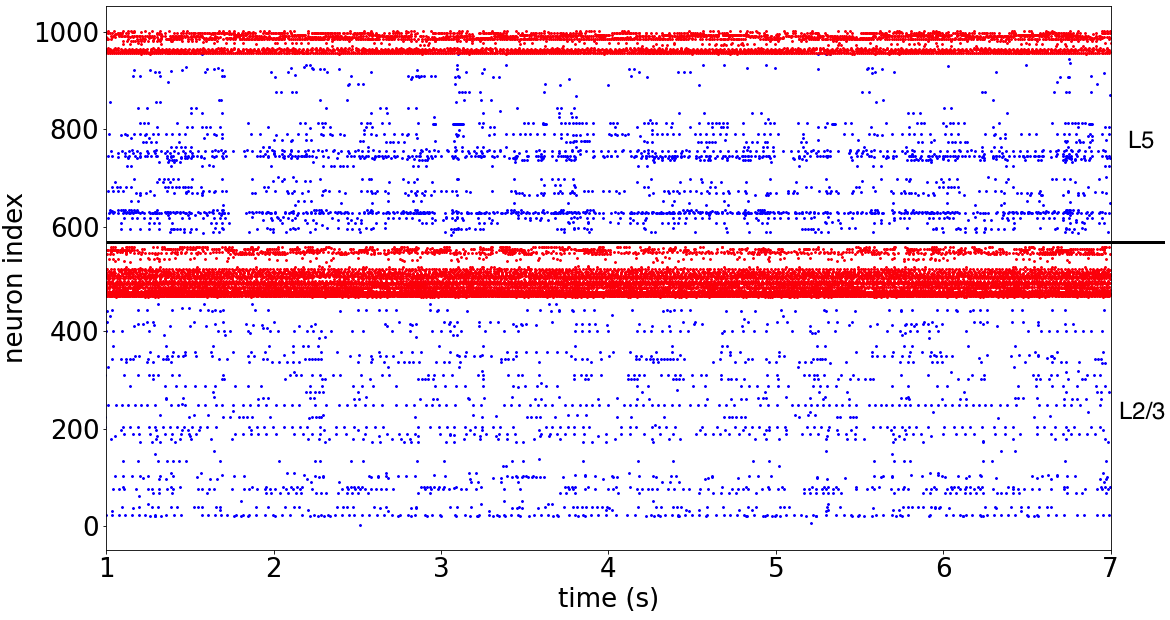
\includegraphics[scale=0.30]{Figures/Fig1.png}
    \caption{Raster plot of baseline spiking activity. The two layers (L2/3 and L5) are separated by a black dashed line, pyramidal cells are in blue and interneurons are in red.}
    \label{fig:fig1}
\end{figure}

Membrane parameters followed broad distributions with differences among cell types, as one can see in Table \ref{tab:membparams}. We further assessed ten independent 30 s baseline simulations to evaluate differences in the rheobase current $I_{SN}$ and the membrane and synaptic parameters between spiking and non-spiking cells in the whole column. The same comparison was made exclusively for the PC cells, either only from L2/3 or only from L5, and also for the two layers together. As in the original work, the rheobase current was significantly lower for spiking cells in all simulations (see Table \ref{tab:tab5}). We also found neurons with negative rheobase, corresponding to ``spontaneous generators''.\\

\begin{table}
    \centering
    \resizebox{\columnwidth}{!}{%
    \begin{tabular}{|c|c|c|c|c|c|c|c|} 
     \hline
     Parameter & PC L2/3 & PC L5 & FS & BT & BC & MC \\[2pt]
    \hline\hline
     $C$ (pF) & 165.28 $\pm$ 55.06 & 246.67$\pm$ 69.02  & 59.67 $\pm$ 11.08 & 81.33 $\pm$ 14.32 & 196.79 $\pm$ 67.24 & 89.98 $\pm$ 20.96  \\[1pt]
    \hline
    $g_L$ (nS) & 7.09 $\pm$ 1.65 & 7.39 $\pm$ 1.62 & 5.40 $\pm$ 0.82 & 3.98 $\pm$ 0.45 & 7.68 $\pm$ 1.76 & 2.86 $\pm$ 0.45 \\[1pt]
    \hline
     $E_L$ (mV) & -84.39 $\pm$ 4.49 & -79.95 $\pm$ 6.34 & -86.36 $\pm$ 4.59 & -83.57 $\pm$ 3.80 & -82.97 $\pm$ 4.79 & -70.78 $\pm$ 6.95 \\[1pt]
    \hline
     $\Delta_T$ (mV) & 21.88 $\pm$ 5.52 &  24.25 $\pm$ 4.88 & 20.20 $\pm$ 7.57 & 19.99 $\pm$ 4.13 & 23.29 $\pm$ 4.74 & 24.75 $\pm$ 10.63   \\[1pt]
    \hline
     $V_T$ (mV) & -51.75 $\pm$ 4.94 & -48.95 $\pm$ 5.95 & -58.71 $\pm$ 6.81 & -59.54 $\pm$ 3.95 & -50.96 $\pm$ 5.06  & -36.33 $\pm$ 5.96 \\[1pt]
     \hline
     $V_{up}$ (mV) & -45.02 $\pm$ 6.67 & -44.20 $\pm$ 6.20 & -50.07 $\pm$ 4.77 & -54.35 $\pm$ 3.64 & -45.95 $\pm$ 5.76  & -36.86 $\pm$ 2.36 \\[1pt]
    \hline
     $V_r$ (mV) & -108.30 $\pm$ 34.36  & -67.62 $\pm$ 12.26 & -85.95 $\pm$ 11.85 & -136.92 $\pm$ 43.20 & -89.43 $\pm$ 31.93   & -54.13 $\pm$ 8.60 \\[1pt]
    \hline
     $b$ (pA)  &  7.27 $\pm$ 5.769  & 6.19 $\pm$ 9.60 & 28.48 $\pm$ 32.77 & 6.59 $\pm$ 9.13 &  5.91 $\pm$ 5.33 & 3.60 $\pm$ 2.62 \\[1pt]
    \hline
    $\tau_w$ (ms) & 112.02 $\pm$ 36.76  & 97.91 $\pm$ 104.49  & 15.27 $\pm$ 2.14 & 44.07 $\pm$ 16.76 & 104.49 $\pm$ 37.76 & 62.31 $\pm$ 14.21 \\[1pt]
    \hline
    
    \hline
    
    \end{tabular}%
    }
    \caption{Mean and standard deviation values of the Gaussian distributions for each one of the membrane parameters. FS (fast-spiking cells): IN-L and IN-L-d; BT (bitufted cells): IN-CL and IN-CL-AC; BC (basket-cells): IN-CC; MC (Martinotti cells): IN-F.}
    \label{tab:membparams}
\end{table}


\begin{table}
    \centering
    \resizebox{\columnwidth}{!}{%
    \begin{tabular}{|c|c|c|c|} 
     \hline
     Group & spiking & $I_{SN}$ (pA) & p-value\\[2pt]
    \hline\hline
    \multirow{2}{*}{Whole column} & Spiking  & 29.613 $\pm$ 34.059 (-80.221 to 120.855) & \multirow{2}{*}{\textit{U} $< 10^{-3}$}\\[1pt]
    \cline{2-3}
    & Not-spiking & 66.205 $\pm$ 40.930 ( -61.102 to 214.506) & \\[1pt]
    \hline\hline
    \multirow{2}{*}{PC L2/3} & Spiking & 51.601 $\pm$ 32.901 ( -7.721 to 114.908) & \multirow{2}{*}{\textit{U} $< 10^{-3}$}\\[1pt]
    \cline{2-3}
    & Not-spiking & 75.299 $\pm$ 38.034 ( -35.807 to 214.506) & \\[1pt]
    \hline\hline
    \multirow{2}{*}{PC L5} & Spiking  & 21.257 $\pm$ 33.921 ( -80.221 to 77.792) & \multirow{2}{*}{\textit{U} $< 10^{-3}$}\\[1pt]
    \cline{2-3}
    & Not-spiking & 55.163 $\pm$ 41.004 ( -61.102 to 203.092) & \\[1pt]
    \hline\hline
    \multirow{2}{*}{PC} & Spiking  & 31.602 $\pm$ 36.528 (-80.221 to 114.908) &  \multirow{2}{*}{\textit{U} $< 10^{-3}$}\\[1pt]
    \cline{2-3}
    & Not-spiking & 66.790 $\pm$ 40.555 (-61.102 to 214.506) &\\[1pt]
    \hline
    \end{tabular}%s
    }
    \caption{Statistics and comparison of rheobase current ($I_{SN})$ between spiking (spike rate $>$ 0.33 Hz) and non-spiking (spike rate $\leq$ 0.33 Hz) cells in the whole column (top row). The 2nd, 3rd and 4th rows show the same values exclusively for PC cells in, respectively, L2/3, L5 and the two layers lumped together. All data were obtained for baseline simulations of 30 s. \textit{U}: Mann-Whitney \textit{U} test.}
    \label{tab:tab5}
\end{table}

In regard to the network parameters, we compared spiking and non-spiking cells parameters using the Mann-Whitney U-test with significance of 0.05, as some parameter distributions are not normally distributed. In the original article, the authors mention that only those parameters related to the rheobase current were significantly different. In our simulations, we found that lower $V_T$ values were associated to lower rheobase current (as expected from equation (\ref{eqn:rheobase})). Moreover, in all the assessed simulations the spiking PCs had lower $V_{\text{up}}$ values than the non-spiking PCs, and this favors the spiking event. In most simulations we also found, associated to spiking PCs in comparison to non-spiking PCs: higher values of $E_L$, which contribute to lower $I_{SN}$ (equation (\ref{eqn:rheobase})); higher values of $\tau_{\text{rec}}^{\scaleto{\text{GABA}}{3pt}}$ and lower values of $\tau_{\text{fac}}^{\scaleto{\text{GABA}}{3pt}}$ in the incoming synapses, which reduce $g_{\scaleto{\text{GABA}}{3pt}}$ and facilitate spiking; and lower values of $g_{\text{GABA}}^{\scaleto{\text{max}}{3pt}}$ in L2/3. Interestingly, we also found lower $\Delta_T$ values in spiking L2/3 PCs in most simulations, which, at least in principle, would lead to a greater rheobase and a lower firing rate. This paradox may be due to the complex interaction among spiking neurons in the network, since lower $\Delta_T$ values cause stronger voltage amplifications when $V > V_T$ (see equation (\ref{eqn:dvdt})).\\

Comparing the connection probabilities $p_{\text{con}}$ for excitatory and inhibitory synapses using the chi-squared test with significance of 0.05, we did not find significant differences between spiking and not-spiking neurons.\\

We analysed the spiking statistics of the network based on a 60 s baseline simulation (see Figure~\ref{fig:fig2}). The distribution of the mean ISI of individual neurons (Figure~\ref{fig:fig2}(a)) is monotonically decreasing with a heavy tail and mean and standard deviation of comparable sizes ($523 \pm 655 \text{ ms}$, mean $\pm$ SD). The distribution of the $C_V$s of ISIs (Figure~\ref{fig:fig2}(b)) has a mean value close to one ($1.13 \pm 0.49$, mean $\pm$ SD). The Pearson cross-correlations between spiking neuron pairs has very low values, with a peak around lag zero and a fast decay for both positive and negative lag values (Figure~\ref{fig:fig2}(c)). For lag zero, the cross-correlation between spiking neuron pairs is $9.7 \times 10^{-4} \pm 6.7 \times 10^{-3}$ (mean $\pm$ SD). The autocorrelation (Figure~\ref{fig:fig3}(a)) has a peak at lag 0, a fast decay and a trough between 0 and 5ms (see the graph in Figure~\ref{fig:fig3}(b)) and then remains near zero.  These results, in agreement with the original article, are consistent with an asynchronous irregular state.\\

\begin{figure}[H]
    \centering
    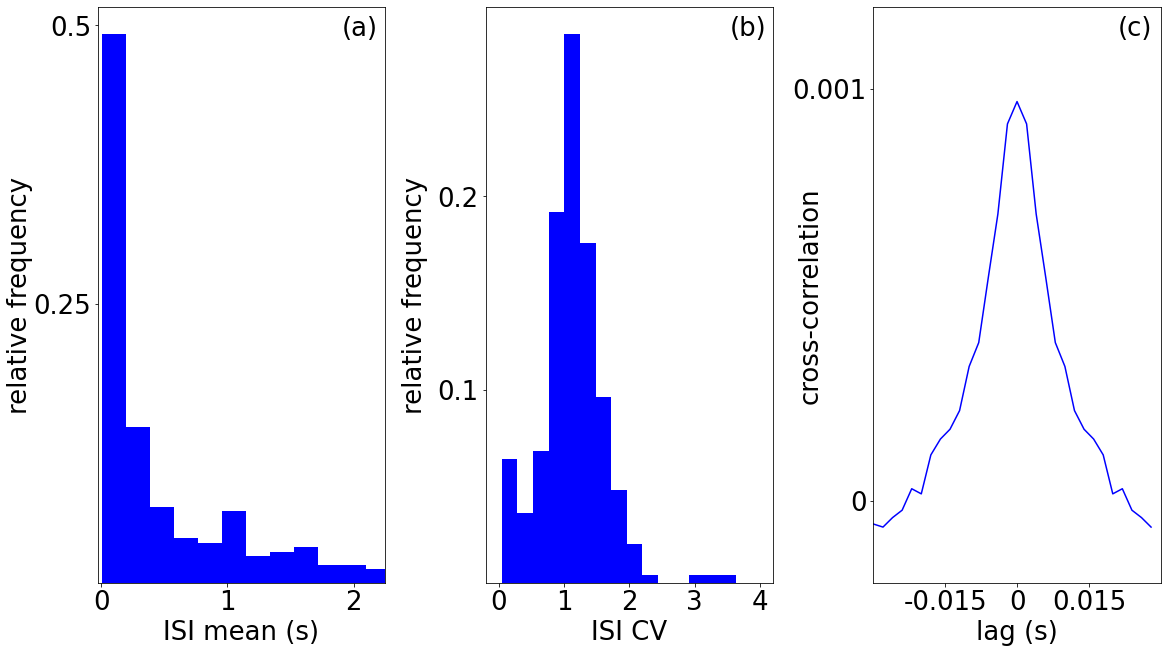
\includegraphics[scale=0.3]{Figures/Fig2.png}
    \caption{(a) Histogram of mean ISIs of spiking neurons. (b) Histogram of $CV_{\text{ISI}}$ values of spiking neurons. (c) Mean Pearson cross-correlation averaged across 200 pairs of spiking neurons.}
    \label{fig:fig2}
\end{figure}

\begin{figure}[H]
    \centering
    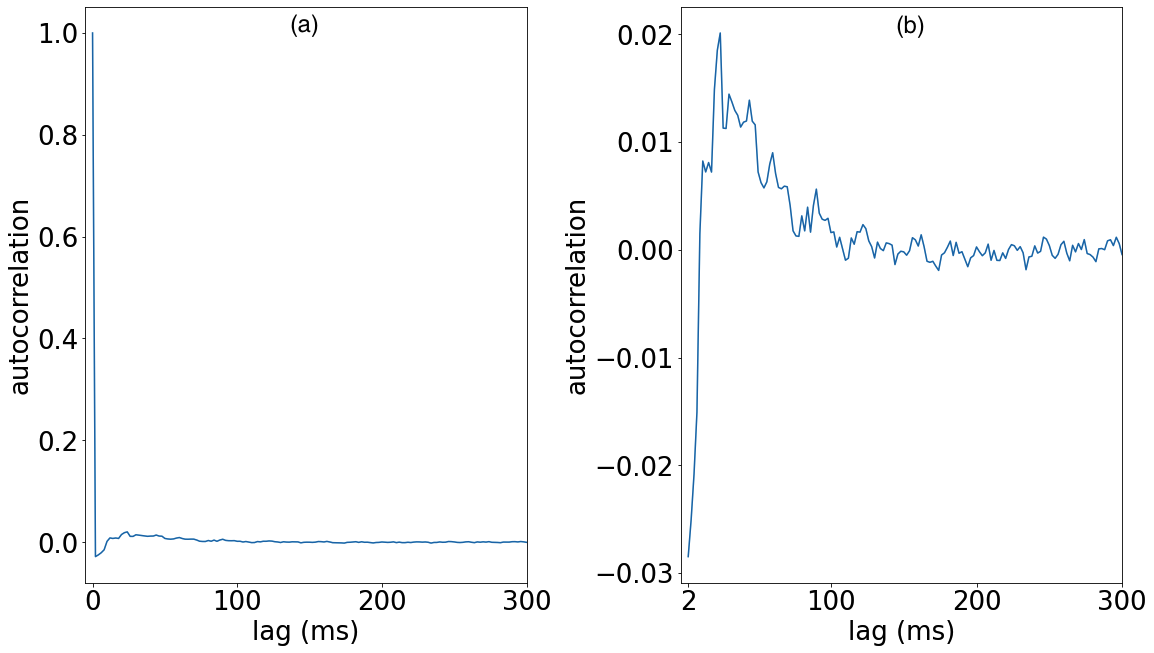
\includegraphics[scale=0.3]{Figures/Fig3.png}
    \caption{(a) Mean autocorrelation of ISIs of spiking neurons. (b) Same plot as in (a) with increased scale of vertical axis and origin of horizontal axis shifted to 2 ms.}
    \label{fig:fig3}
\end{figure}

We estimated the LFP from a 30 second baseline simulation as described in Methods (Figure \ref{fig:LFP}). In agreement with the original article, we found an approximate power-law distribution ($P \approx 1/f^{\alpha}$) with $\alpha \approx 1$ for frequencies below 60 Hz %($\approx 4.09 \text{ log}([Hz])$ 
and $2 < \alpha < 3$ for frequencies above 60 Hz (Figure \ref{fig:LFP}).\\

\begin{figure}[H]
    \centering
    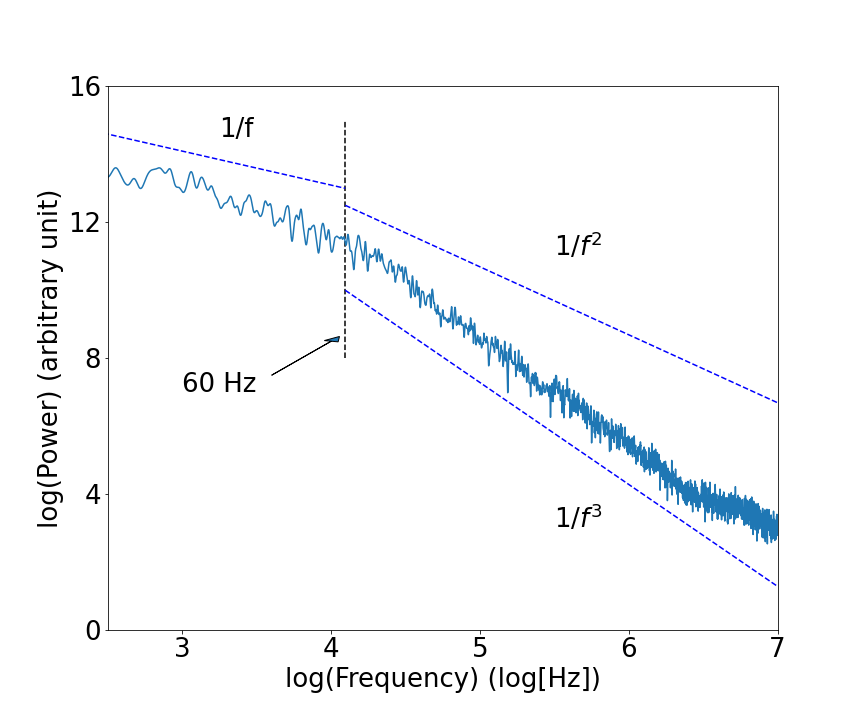
\includegraphics[scale=0.25]{Figures/Fig4.png}
    \caption{Power spectrum of the LFP of baseline activity.}
    \label{fig:LFP}
\end{figure}

Also in agreement with the original article, spiking neurons displayed a broad range of membrane potential fluctuations. After removing spike events as described in Methods, the standard deviation of the membrane potentials of spiking neurons was $2.82 \text{ mV } \pm 1.43 \text{ mV}$ (mean $\pm$ std) for the whole column (Figure \ref{fig:fig5}(a)), and $2.42 \text { mV } \pm 0.94 \text{ mV}$ (mean $\pm$ std) for pyramidal cells only (Figure \ref{fig:fig5}(b)).

\begin{figure}[H]
    \centering
    \begin{minipage}[b]{0.45\textwidth}
    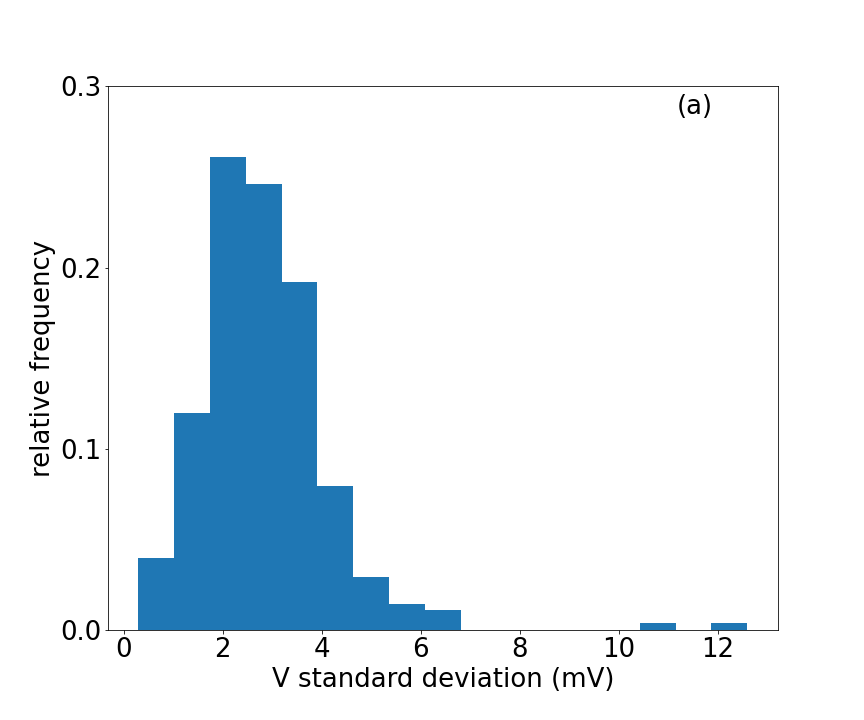
\includegraphics[scale=0.23]{Figures/Fig5a.png}
    \end{minipage}
    \hfill
    \begin{minipage}[b]{0.5\textwidth}
        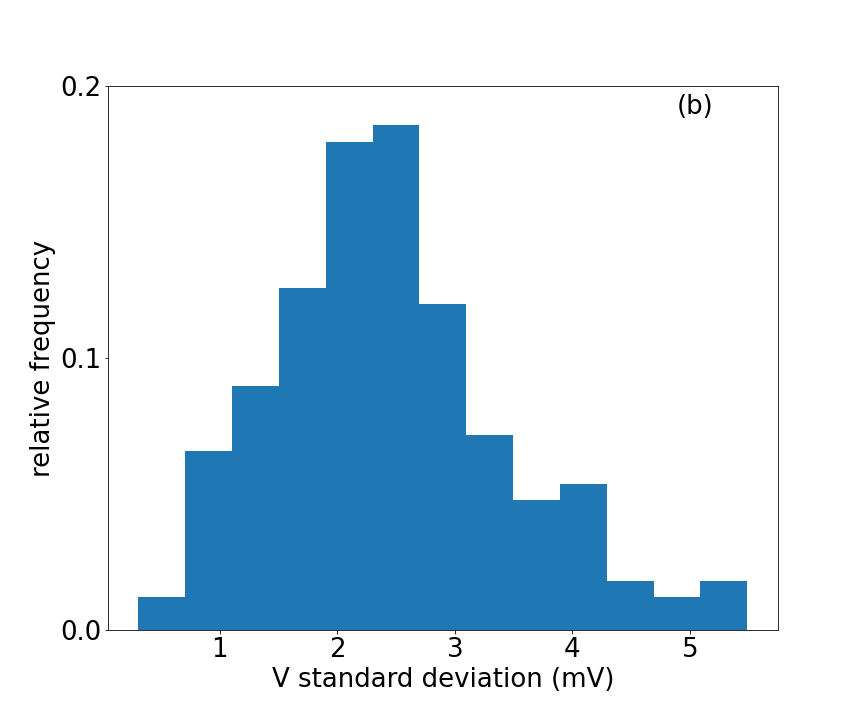
\includegraphics[scale=0.23]{Figures/Fig5b.png}
    \end{minipage}
    \caption{(a) Histogram of standard deviations of the membrane potentials of individual spiking neurons in the whole column. (b) Same as in (a) but only for pyramidal cells.}
    \label{fig:fig5}
\end{figure}

For a more consistent comparison, we performed the same spike statistics and LFP analyses as above in a 60 s baseline simulation of the original MATLAB code available in the ModelDB repository (\url{https://senselab.med.yale.edu/ModelDB/ShowModel?model=189160#tabs-1}). The results are shown in Figures (\ref{fig:fig6}), (\ref{fig:fig7}) and (\ref{fig:fig8}) and are in good quantitative agreement with the ones shown in Figures (\ref{fig:fig2}), (\ref{fig:fig3}) and (\ref{fig:LFP}), respectively. The numerical values for the simulation of the original MATLAB code are: mean ISI ($516 \text{ ms } \pm 680 \text{ ms}$, mean $\pm$ std); CV$_{\text{ISI}}$ ($1.10 \pm 0.45$, mean $\pm$ std); and zero-lag value of the Pearson cross-correlation between neuron pairs ($6.7 \times 10^{-4} \pm 6.5 \times 10^{-3}$, mean $\pm$ SD). \\

\begin{figure}[H]
    \centering
    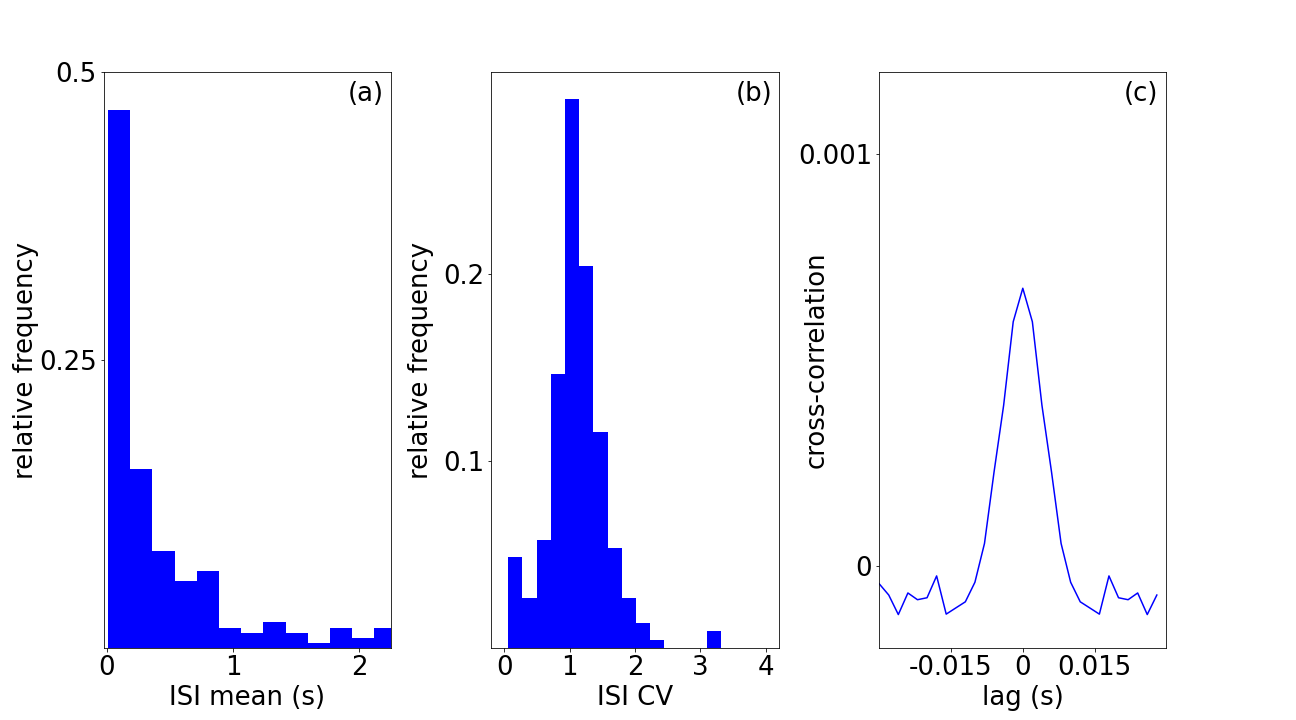
\includegraphics[scale=0.30]{Figures/Fig6.png}
    \caption{Spike statistics for a simulation of the original MATLAB code. (a) Histogram of mean ISIs of spiking neurons. (b) Histogram of $CV_{\text{ISI}}$ values of spiking neurons. (c) Mean Pearson cross-correlation averaged across 200 pairs of spiking neurons.}
    \label{fig:fig6}
\end{figure}

\begin{figure}[H]
    \centering
    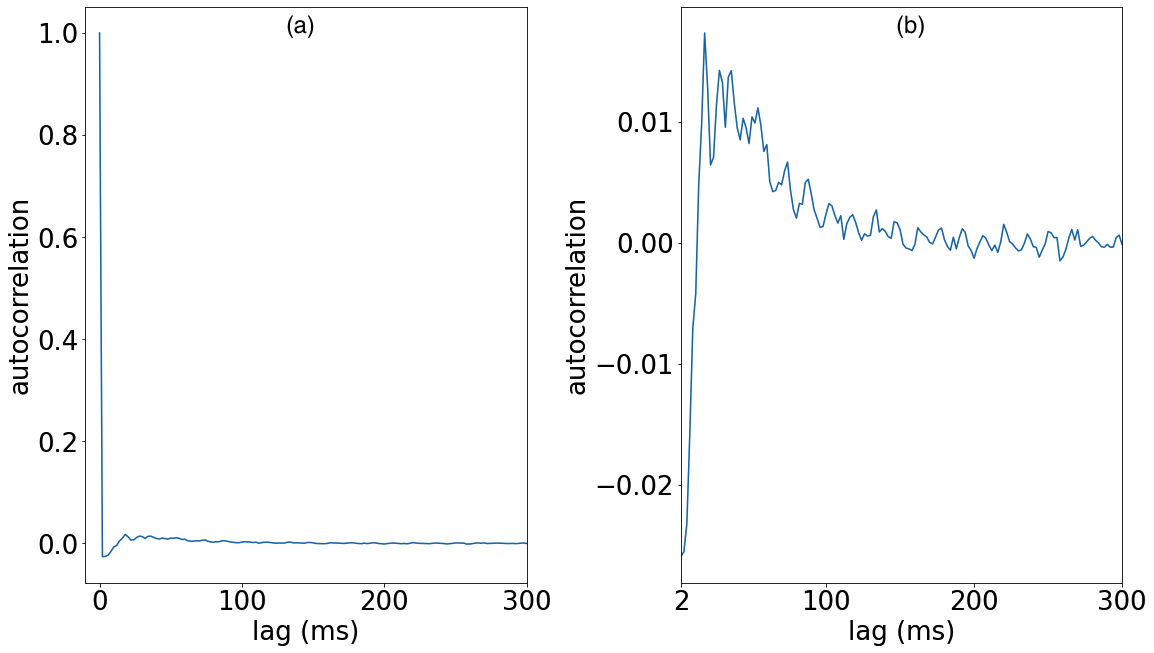
\includegraphics[scale=0.30]{Figures/Fig7.png}
    \caption{(a) Mean autocorrelation of ISIs of spiking neurons for a simulation of the original MATLAB code. (b) Same as in (a) with increased scale of vertical axis and origin of horizontal axis shifted to 2 ms.}
    \label{fig:fig7}
\end{figure}

\begin{figure}[H]
    \centering
    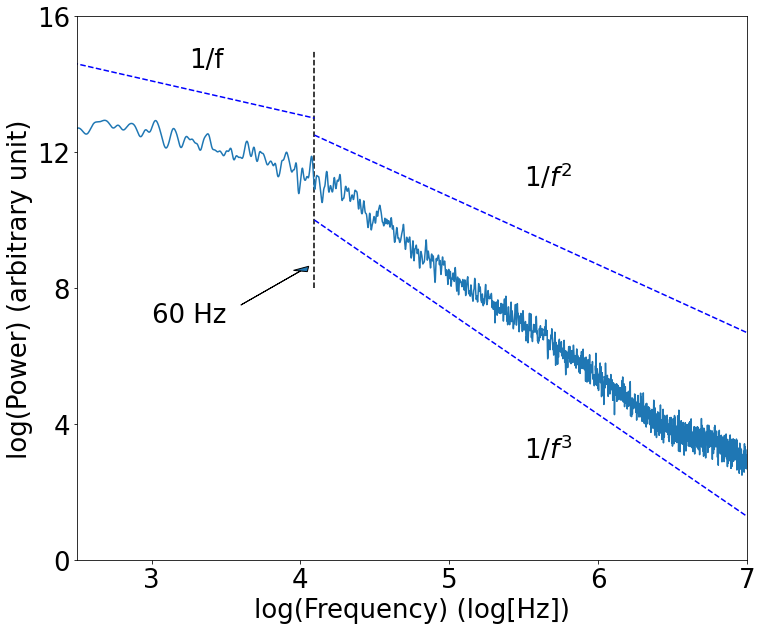
\includegraphics[scale=0.3]{Figures/Fig8.png}
    \caption{Power spectrum of the LFP of baseline activity for a simulation of the original MATLAB code.}
    \label{fig:fig8}
\end{figure}

We also performed the above analyses solving the EDOs with the Brian2 gsl\_rk2 algorithm, which implements a second order Runge-Kutta method with adaptive time step. The results are in good quantitative agreement with the two replications presented above. A raster plot of spiking activity can be seen in Figure \ref{fig:fig9} and the plots for the spiking statistics and power spectrum can be seen in Figures (\ref{fig:fig10}), (\ref{fig:fig11}) and (\ref{fig:fig12}). The numerical values are: mean ISI ($511 \text{ ms } \pm 665 \text{ ms}$, mean $\pm$ SD); CV$_{\text{ISI}}$ ($0.97 \pm 0.45$, mean $\pm$ SD); and zero-lag value of the Pearson cross-correlation between neuron pairs ($7.0 \times 10^{-4} \pm 6.4 \times 10^{-3}$).\\ 

\begin{figure}[H]
    \centering
    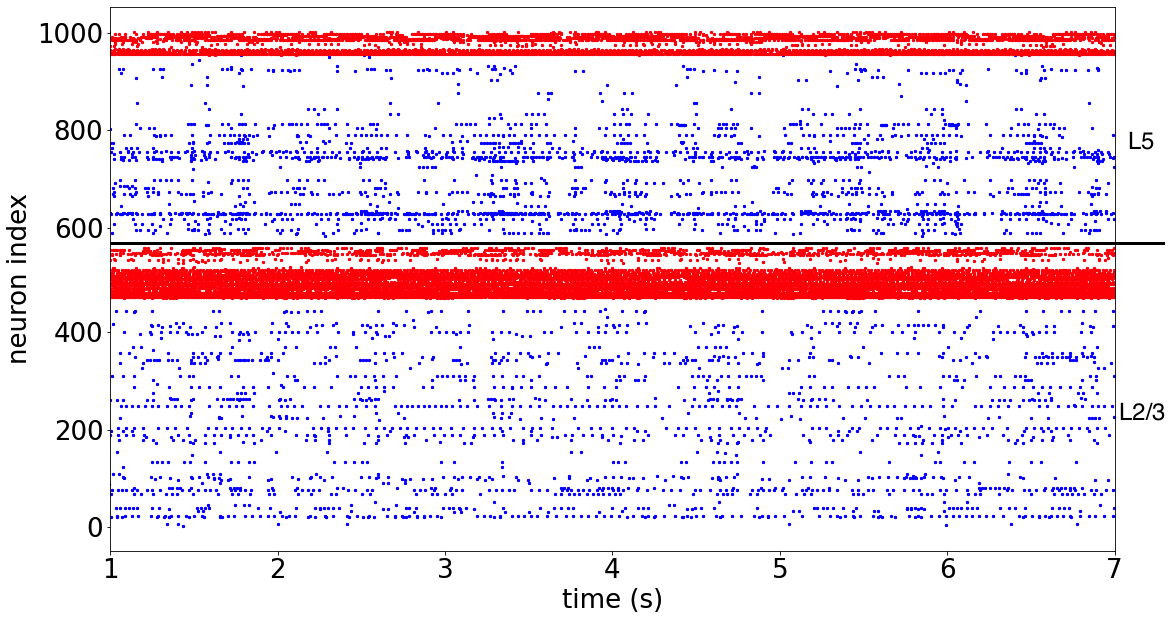
\includegraphics[scale=0.3]{Figures/Fig9.png}
    \caption{Raster plot of baseline spiking activity obtained with Brian2 gsl\_rk2 algorithm.}
    \label{fig:fig9}
\end{figure}

\begin{figure}[H]
    \centering
    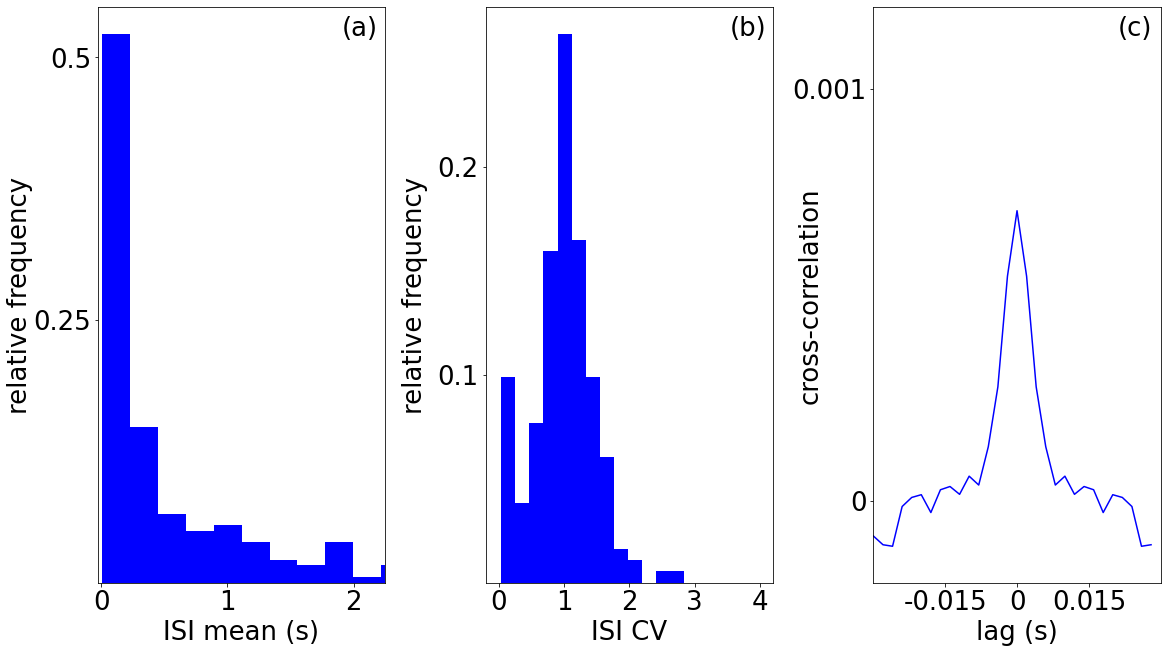
\includegraphics[scale=0.3]{Figures/Fig10.png}
    \caption{Spike statistics for the simulation of the model using the Brian gsl\_rk2 algorithm. (a) Histogram of mean ISIs of spiking neurons. (b) Histogram of $CV_{\text{ISI}}$ values of spiking neurons. (c) Mean Pearson cross-correlation averaged across 200 pairs of spiking neurons.}
    \label{fig:fig10}
\end{figure}

\begin{figure}[H]
    \centering
    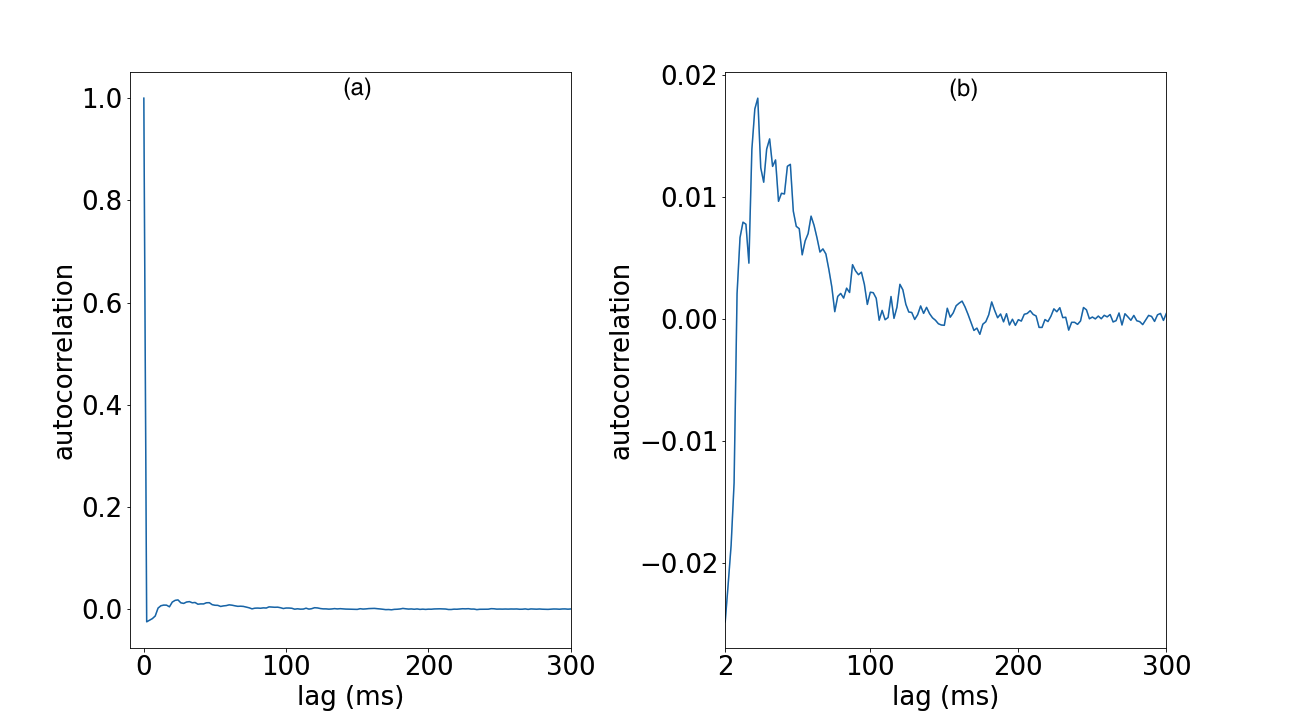
\includegraphics[scale=0.3]{Figures/Fig11.png}
    \caption{(a) Mean autocorrelation of ISIs of spiking neurons for the simulation of the model using the Brian gsl\_rk2 algorithm. (b) Same as in (a) with increased scale of vertical axis and origin of horizontal axis shifted to 2 ms.}
    \label{fig:fig11}
\end{figure}

\begin{figure}[H]
    \centering
    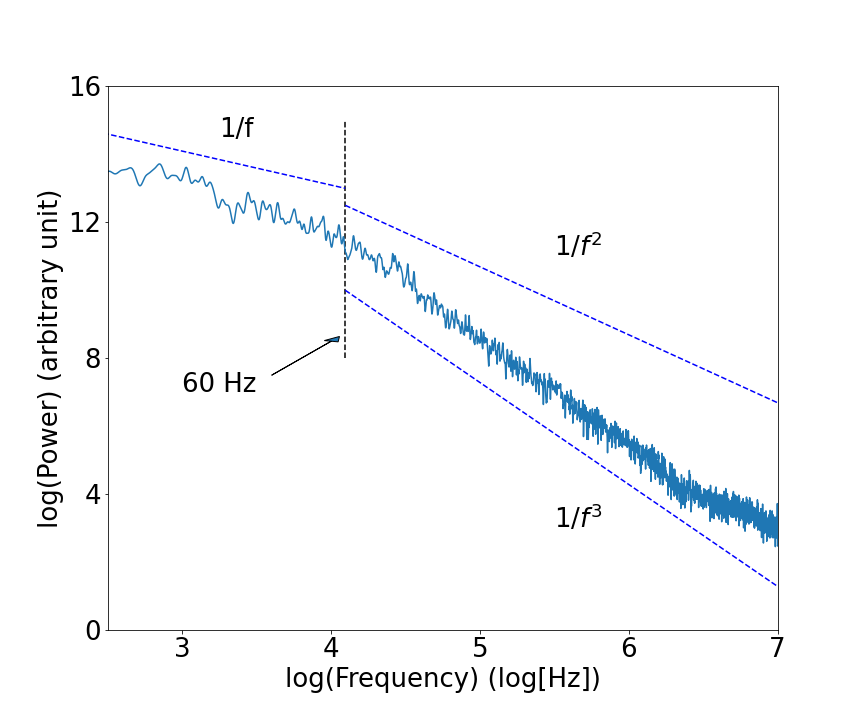
\includegraphics[scale=0.3]{Figures/Fig12.png}
    \caption{Power spectrum of the LFP of baseline activity for the simulation of the model using the Brian gsl\_rk2 algorithm. }
    \label{fig:fig12}
\end{figure}

We next investigated the L2/3 and L5 responses to brief regular stimuli (see Stimulation protocols in Methods). We applied 250 regular spikes to 10\% of the PCs in L2/3 with synaptic strength $g_{\text{syn}}$ = 0.1 nS. This induced a strong activation of the L2/3 cells after 3-4 ms followed by an activation of the L5 cells after 11-12 ms of the stimulus onset (Figure \ref{fig:fig13}(a)). These two delays are greater than what would be expected from the individual synaptic delay $\tau_D$ (synapses to PCs have $\tau_D$s with mean $\pm$ std equal to 1.82 ms $\pm$ 0.74 ms and 1.74 ms $\pm$ 0.39 ms in L2/3 and L5, respectively), suggesting that they depend on network rather than single-cell dynamics. For a stronger stimulation consisting of 500 regular spikes within 5 ms, we observed a faster and longer activation of the L2/3 cells; on the other hand, the activation of the L5 cells was also faster but the duration was shorter (Figure \ref{fig:fig13}(b)).\\

\begin{figure}[H]
    \centering
    \begin{minipage}[b]{0.45\textwidth}
    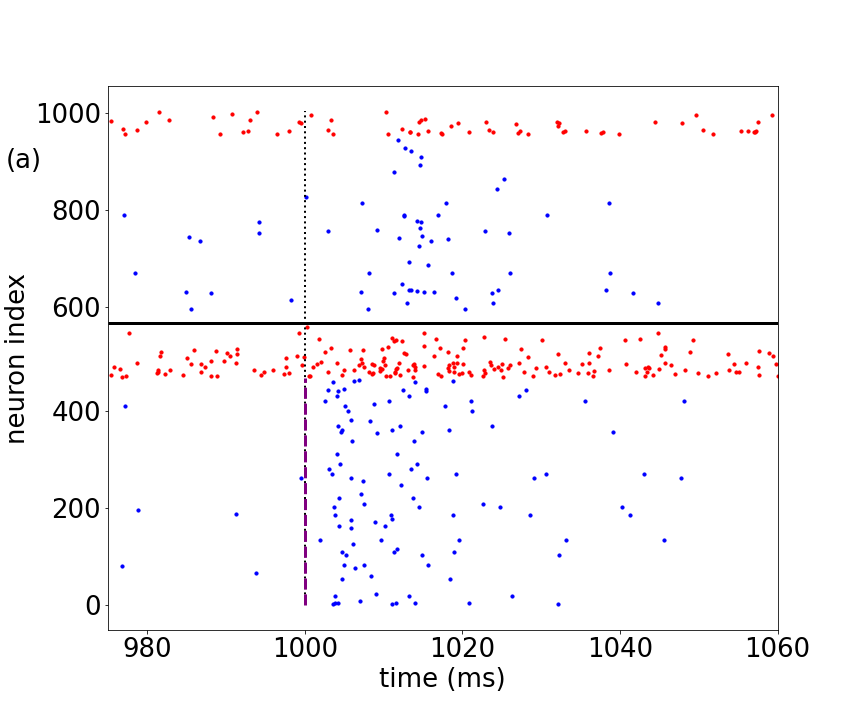
\includegraphics[scale=0.23]{Figures/Fig13a.png}
    \end{minipage}
    \hfill
    \begin{minipage}[b]{0.5\textwidth}
        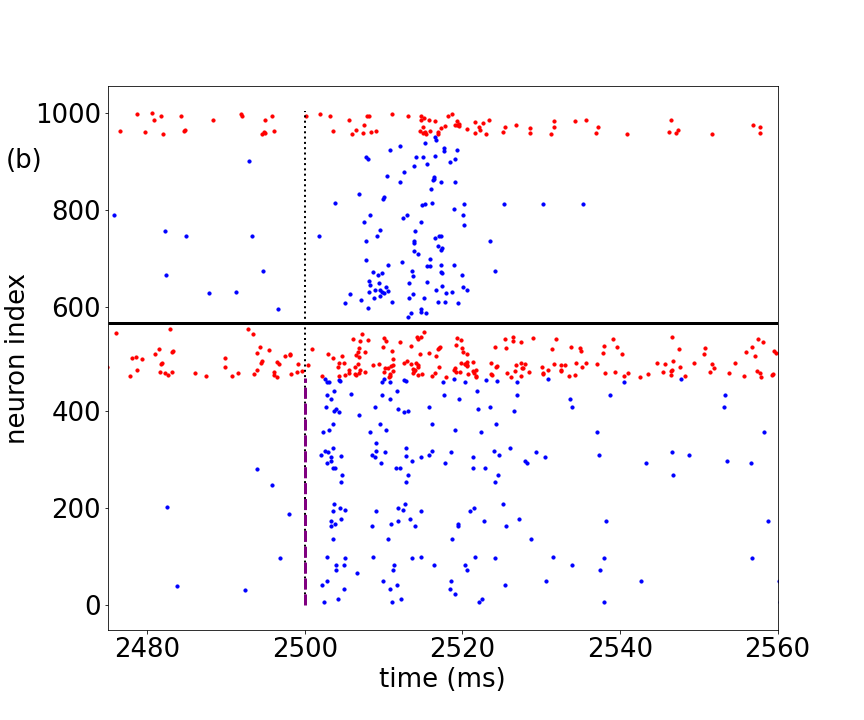
\includegraphics[scale=0.23]{Figures/Fig13b.png}
    \end{minipage}
    \caption{Propagation of transient input. (a) Raster plot of spiking activity in response to an external input (dashed line) to 10\% of the PCs in L2/3 consisting of 250 spikes in 5 ms. (b) same as in (a) but the with 500 spikes in 5ms.}
    \label{fig:fig13}
\end{figure}

To examine the dependence of network dynamics on neuronal heterogeneity, we analyzed the propagation of transient input in a network with reduced  parameter variability (but no change in the means). For a reduction to 20\% of the original value in the the standard deviation of all the membrane parameters, the response of the L2/3 cells was similar to the one without variability but the response of the L5 cells was significantly weaker (Figure \ref{fig:fig14}). As shown in Figure \ref{fig:fig15}, the response (defined as the number of spikes in the first 50 ms after stimulus onset) of L5 PCs to a brief transient input is more strongly affected by the variability of membrane parameters than the response of L2/3 PCs. \\

\begin{figure}[H]
    \centering
    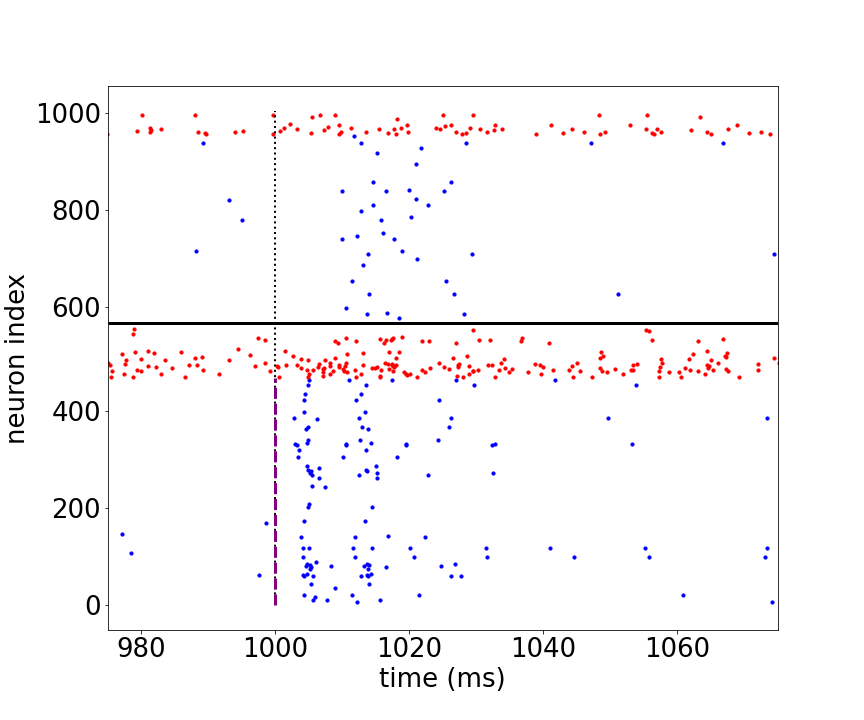
\includegraphics[scale=0.25]{Figures/Fig14.png}
    \caption{Raster plot of spiking activity for the same conditions as in Figure \ref{fig:fig13}(a) but with the standard deviations of the membrane parameters reduced to 20\% of the original values.}
    \label{fig:fig14}
\end{figure}

\begin{figure}[H]
    \centering
    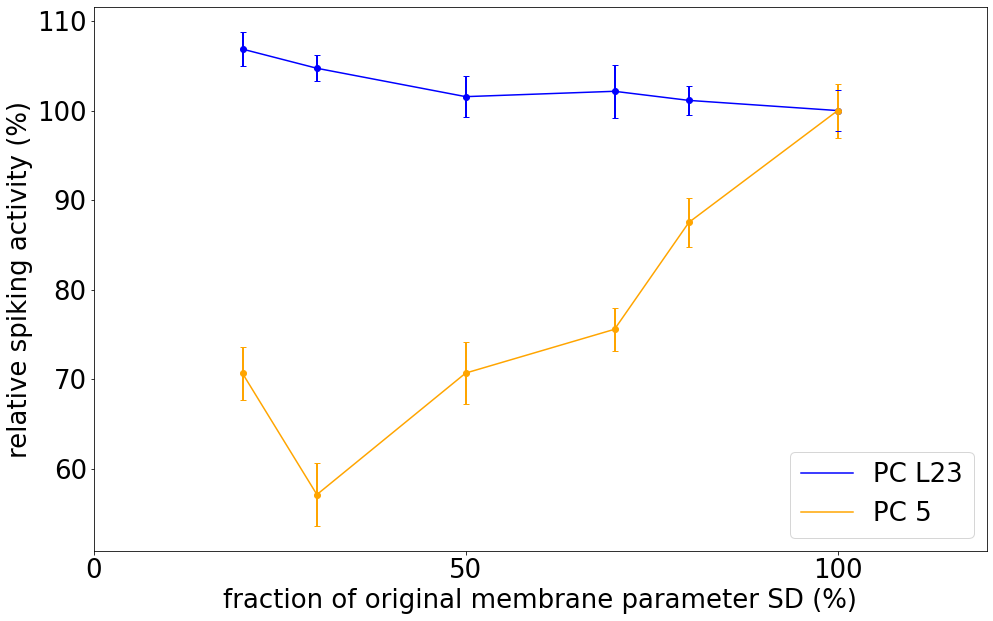
\includegraphics[scale=0.25]{Figures/Fig15.png}
    \caption{Effect of neuronal variability on the response to transient stimuli. Plot of the relative variation of the number of spikes as a function of the percentage of the original standard deviation of neuronal parameters, for PCs in L2/3 and L5. Spiking activity was measured as the spike count during the first 50 ms after stimulus onset. Each data point is the mean $\pm$ SEM over 18 independent simulations.}
    \label{fig:fig15}
\end{figure}

We further investigated whether or not there is bidirectional symmetry in the transmission of stimuli between L2/3 and L5. To do this, we applied Poisson spike trains of 100 ms of duration (as described in Stimulation protocols in Methods) to 10\% of PCs in either L2/3 or L5 and observed the effect on the network. When the stimulation was applied to L2/3 the activation propagated to L5 (Figure~\ref{fig:fig16}(a)), but when the stimulation was applied to L5 it did not propagate to L2/3 (Figure~\ref{fig:fig16}(b)).\\  

Finally, we studied the impact of suppressed inhibition on the dynamics of the network response to external stimuli. The study was done using the same stimulation protocol of the previous study, with Poisson external stimulation applied to either 10\% of PCs in L2/3 or 10\% of PCs in L5. The difference is that now we reduced the synaptic strengths of all the inhibitory synapses to 40\% of their original value. As can be seen in Figure~\ref{fig:fig17}(a), the stimulation of PCs in L2/3 produced epileptiform activity in both L2/3 and L5. On the other hand, the stimulation of PCs in L5 induced epileptiform activity only in L5 without propagation to L2/3 (Figure~\ref{fig:fig17}(b)).


\begin{figure}[H]
    \begin{minipage}[b]{0.45\textwidth}
    \centering
    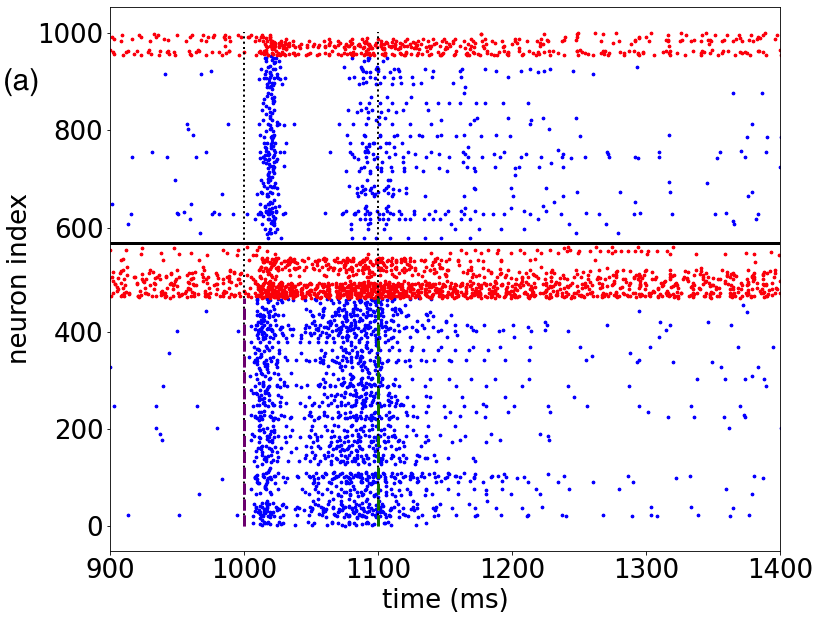
\includegraphics[scale=0.23]{Figures/Fig16a.png}
    \end{minipage}
    \hfill
    \begin{minipage}[b]{0.5\textwidth}
    \centering
    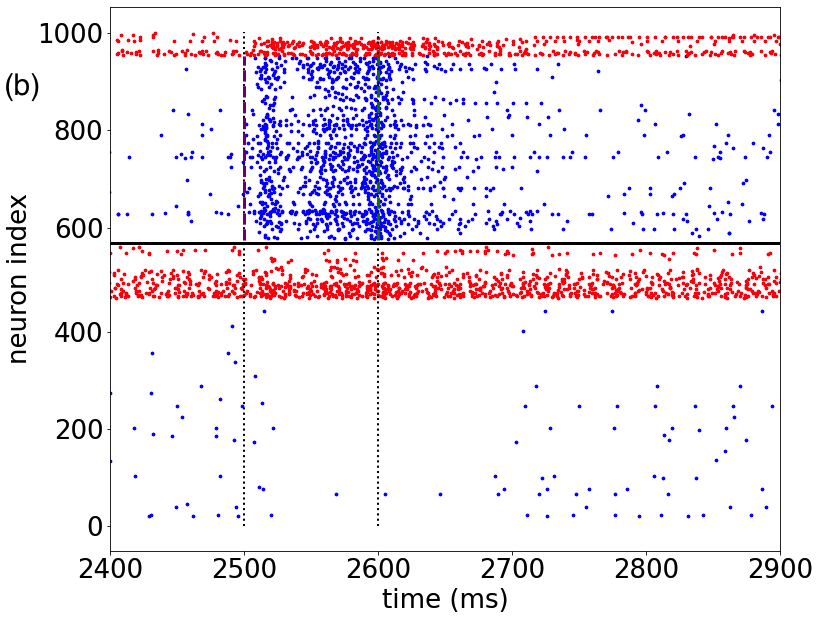
\includegraphics[scale=0.23]{Figures/Fig16b.png}
    \end{minipage}
    \caption{Bidirectional asymmetry in the network. (a) Raster plot of network spiking activity for a Poisson stimulation of 100 ms of duration (indicated by vertical dashed lines) applied to 10\% of PCs in L2/3. (b) Raster plot of network spiking activity for the same type of Poisson stimulation as in (a) applied to 10\% of PCs in L5.}
    \label{fig:fig16}
\end{figure}

\begin{figure}[H]
    \centering
    \begin{minipage}[b]{0.45\textwidth}
    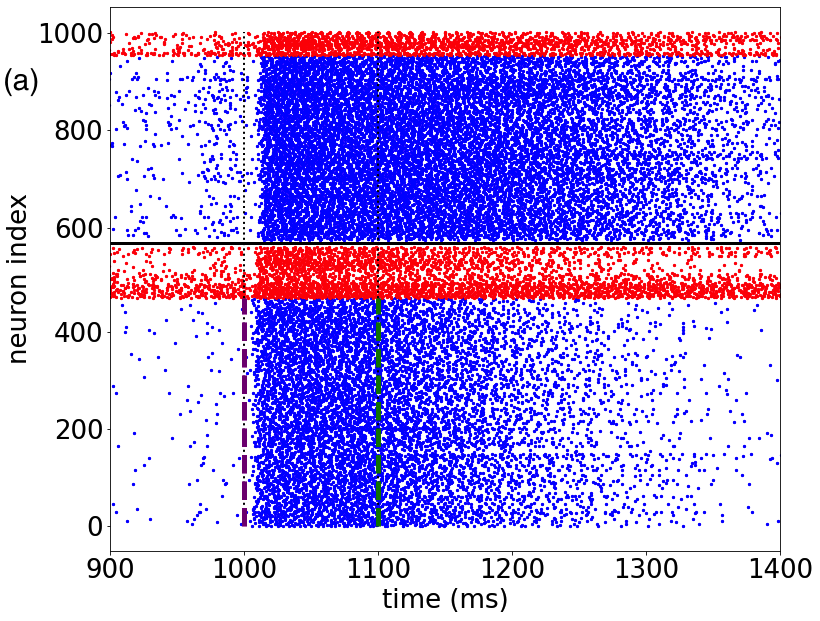
\includegraphics[scale=0.25]{Figures/Fig17a.png}
    \end{minipage}
    \hfill
    \begin{minipage}[b]{0.5\textwidth}
        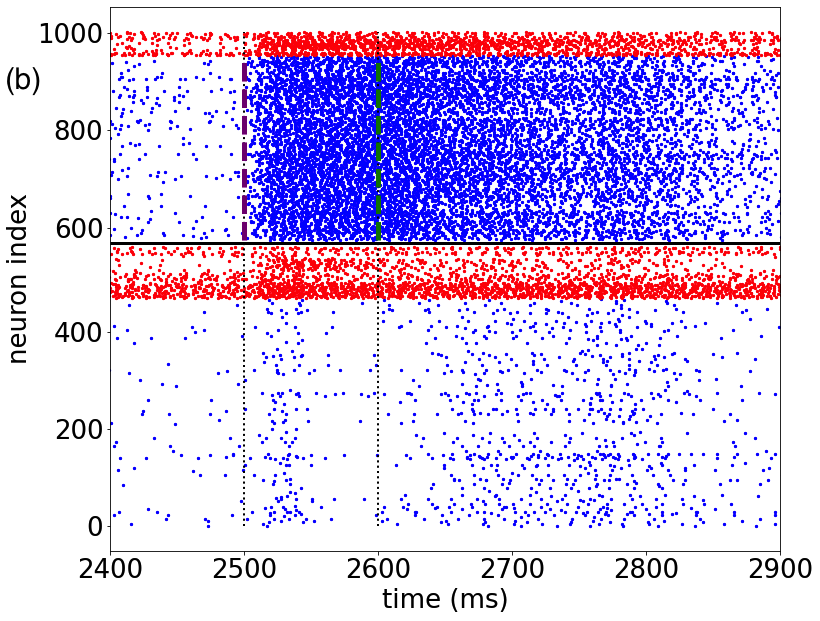
\includegraphics[scale=0.25]{Figures/Fig17b.png}
    \end{minipage}
    \caption{Effect of supressed inhibition on the network activity. The raster plots in (a) and (b) correspond to the same types of stimulation as in Figures~\ref{fig:fig16}(a) and \ref{fig:fig16}(b) but now the synaptic strengths of the inhibitory synapses were reduced to 40\% of the original values.}
    \label{fig:fig17}
\end{figure}

\section*{Conclusions}

We reimplemented the prefrontal cortex model of Hass et al. (2016) \cite{Hass2016} using Python and the Brian 2 package (with two ODE integration methods of different orders of precision). We explained the details of our reimplementation and analyses methods in the hope of clarifying some aspects left unexplained in the original article. We successfully replicated the main features of the original model: 
\begin{itemize}
    \item broad parameter distribution for each cell type;
    \item low fraction of spiking neurons, which display lower rheobase currents than the remaining neurons;
    \item asynchonous and irregular spiking activity;
    \item LFP with $1/f$ behavior for frequencies below 60 Hz and $1/f^{\alpha}$ with $2 < \alpha <3$ for frequencies above 60 Hz; 
    \item latency times and duration of PC activation depending on stimulus strength and network rather than single-cell dynamics;
    \item bidirectional asymmetry in the propagation of stimulus activity between L2/3 and L5;
    \item stronger dependence of L5 PC activation on membrane parameter variability than of L2/3 PC activation;
    \item epileptiform activity triggered by inhibitory strength reduction.
\end{itemize}

\section*{Acknowledgments}

N.L.K. is supported by FAPESP grant 2020/02675-9. A.C.R. is supported by FAPESP grants 2015$/$50122-0 and 2018$/$20277-0, and CNPq grant 303235/2018-7.
This article was produced as part of the activities of FAPESP  Research, Innovation and Dissemination Center for Neuromathematics (Grant No. 2013/07699-0, S. Paulo Research Foundation).